\section{Polarization by Effective Antagonism}\label{sec:er-comparison}

In their seminal paper \cite{esteban1994measurement}, Esteban and Ray laid down three axioms that a measure of polarization should satisfy. They also introduced a parametric measure, which we denote by \ERLabel, and stated that it is the only measure of certain form that satisfies these axioms.

\subsection{The Esteban--Ray Measure}

The Esteban--Ray measure (\ERLabel) is essentially pairwise. It adds up the tension between every pair of groups, weighting opinion difference by group size and by a term emphasizing group identity.

\begin{definition}[Esteban--Ray measure \cite{esteban1994measurement}]\label{ER:measure} The Esteban--Ray measure \(\ERLabel:\Dset \to \PositiveReals\) is given by
\begin{equation}
\ER(\pi) \defsymbol K \sum_{x\in\support(\pi)}\sum_{y\in\support(\pi)}\pi(x)^{1+\alpha}\pi(y)|x - y|,
\end{equation}
where $K > 0$ is a normalization constant, and $\alpha \in (0, \alpha^*]$, with $\alpha^* \approx 1.6$ empirically derived.
\end{definition}
From the results \cite{esteban1994measurement} it follows that \ERLabel{} is a polarization measure in the sense of Def.~\ref{pol:def}. The guiding idea in Def.~\ref{ER:measure} is that polarization grows when there are large groups that are far apart. The $\MEC$ measure also captures this but from a different perspective: It asks what is the least effort needed to bring the whole distribution to a consensus.

The optimization-based character of $\MEC$ yields information that \ERLabel{} does not provide, namely, the optimal consensus points. This is important for two reasons. On the one hand, it supplies a geometric structure that is useful in proving properties such as the increase of polarization under shifts away from optimal consensus (Th.~\ref{thm:mec-increases:body}) or that minorities always bear the greater effort (Th.~\ref{thm:minority-principle-general}). On the other hand, it has a direct social significance, since it indicates the points at which consensus can be achieved with least effort in a given population.

Furthermore, like \ERLabel, $\MEC$ uses the parameter $\alpha$ to reflect group identity. It differs from \ERLabel, however, in introducing a further parameter, $\beta$, which governs how severely distance from consensus is penalized. This not only allows $\MEC$ to distinguish more sharply between moderate and extreme deviations, but also determines the structure of the set of optimal consensus points, since for $\beta>1$ the optimal consensus point is unique, whereas for $\beta=1$ it need not be.

The two measures agree on an important intuition: societies split into two large and distant blocs should be highly polarized. In particular, the symmetric two-extreme distribution $\pi^*$ gives  maximal polarization under both approaches. But they justify this in different ways: \ERLabel{} sees two large hostile camps while $\MEC$ sees the greatest resistance to consensus.

\subsection{The \texorpdfstring{\ERLabel}{ER} Axioms}\label{sec:er-axioms}


Despite proceeding from a different conception of polarization, $\MEC$ satisfies all three of Esteban and Ray's axioms throughout its standing parameter range $\alpha,\beta\geq 1$. The only restriction is that Axiom~1 requires the strict inequality $\alpha>1$. This is not specific to $\MEC$: under the parametrization of \cite{esteban1994measurement}, the mass exponent is $1+\alpha_{\ERLabel}$ with $\alpha_{\ERLabel}>0$, which is the same condition (mass exponent strictly greater than $1$) expressed in a different variable. The strict inequality is, in this sense, intrinsic to the identification dimension of polarization rather than an accident of either formulation. The need for it is also natural in light of Cor.~\ref{cor:mec-special-cases}: when $\alpha=1$, $\MEC$ reduces to a standard dispersion measure (Earth Mover's Distance, mean absolute deviation about a median, or variance), and dispersion measures are known not to capture the consolidation phenomenon described by Axiom~1.



The axioms stated below distill the conceptual insights of Esteban and Ray into precise, testable properties governing how the consolidation of proximate clusters, increased separation among groups, and redistribution of mass toward the extremes should affect a polarization index. They thus serve as normative criteria: any measure that satisfies them faithfully captures the core sociological intuitions about group cohesion and antagonism \cite{kawada2018characterization}.

\paragraph{Axiom 1 (Increased identification).}
The first \ERLabel{} axiom says, in effect, that polarization increases when two groups of size $q$, sufficiently small relative to a larger third group of size $p$ and sufficiently close to one another, are fused into one.

\begin{axiom}[Polarization via increased identification]\label{axiom:1}
A polarization measure $\Pol:\Dset\to \PositiveReals$ satisfies \ERLabel{} Axiom~1 if it satisfies the \emph{increased identification condition}: For any $p>0$ and any $x>0$, there exist $\varepsilon>0$ and $\mu>0$ such that, for all $y>x$ and all $q<p$, if $y-x<\varepsilon$ and $0<q<\mu p$, then
\[
\Pol((p,q,q),(0,x,y)) < \Pol\!\left((p,2q),\left(0,\frac{x+y}{2}\right)\right).
\]
\begin{figure}[H]
    \centering
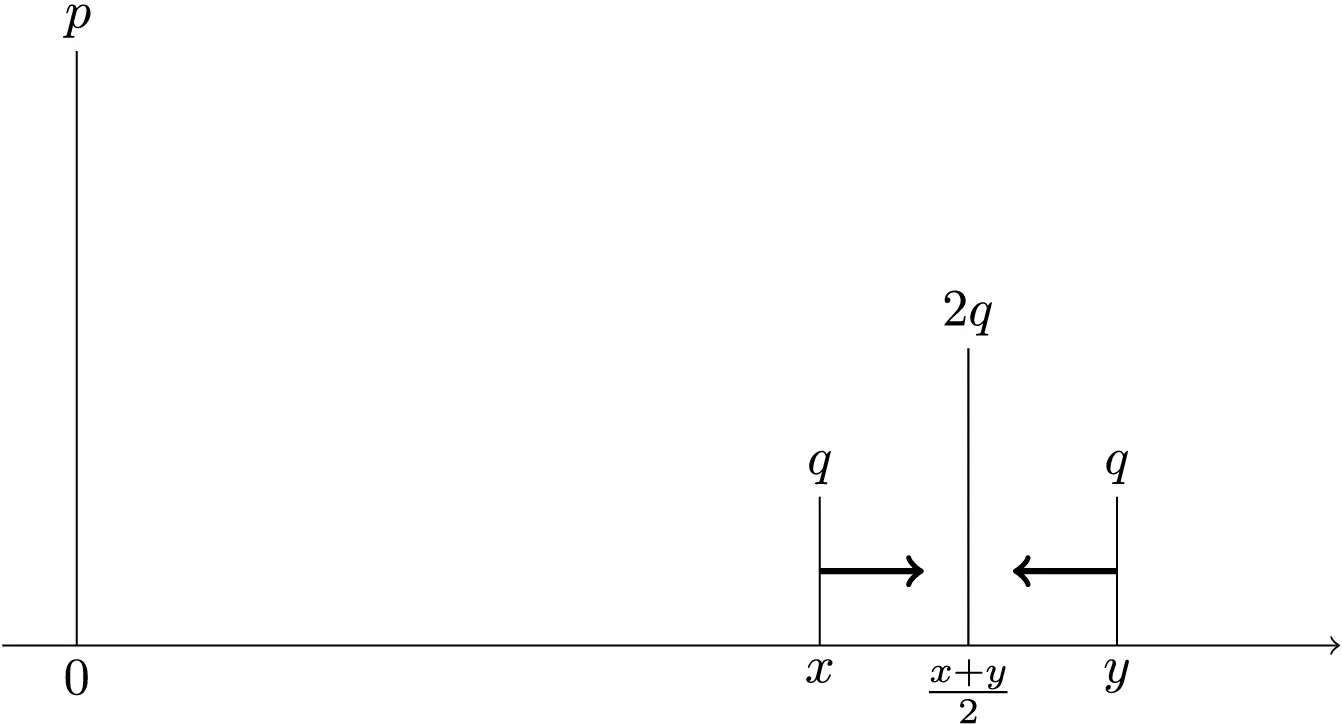
\includegraphics[height=0.16\textheight,keepaspectratio]{Images/er_axioms/axiom1.png}
    \caption{Esteban--Ray Axiom 1.}
    \label{fig:eraxiom1}
\end{figure}
\end{axiom}

\noindent Intuitively, consolidating smaller, closely positioned groups into fewer, larger groups enhances identification and thus polarization.

It turns out that the condition $\alpha>1$ is not merely sufficient, but also necessary, for our $\MEC$ functions to satisfy Axiom~1.

\begin{restatable}{theorem}{mecAxiomOne}\label{th:mec-axiom-1} The polarization measure $\MEC$ satisfies Axiom~1 if and only if $\alpha > 1$.
\end{restatable}

An immediate consequence of this theorem is that the instances $\MEC[1,1]$ and $\MEC[1,2]$ do not satisfy Axiom~1. In view of Th.~\ref{th:mec-as-emd} and Cor.~\ref{cor:mec-special-cases}, these correspond to well-known probabilistic measures, namely Earth Mover's Distance, the mean absolute deviation about a median, and the variance.

The proof of Th.~\ref{th:mec-axiom-1} compares the effort functions of 
\(\pi=((p,q,q),(0,x,y))\) and the merged distribution
\(\tilde\pi=((p,2q),(0,(x+y)/2))\). Writing \(h=y-x\), the difference of these functions at a
point \(z\in(0,x)\) can be written as \(q^\alpha\Delta(A,h)\), where
\(A=x-z\). The quantity \(\Delta(A,h)\) splits into two parts: a non-negative
term coming from the convexity of \(t\mapsto t^\beta\), and a negative term
proportional to \(2^\alpha-2\), which measures the gain in identification
produced by merging the two masses \(q\) and \(q\) into a single mass \(2q\).

The smallness of the mass \(q\) with respect to $p$ ensures that the relevant optimal consensus points lie near the mass \(p\) at \(0\), so that the
comparison is made in the right region. When \(\beta>1\), the smallness of the distance
\(h\) ensures that the positive convexity term remains controlled. If
\(\alpha>1\), the negative identification term is present and, for small enough
\(h\), it dominates; hence the merged distribution has larger MEC. If
\(\alpha=1\), this term disappears. One then gets equality when \(\beta=1\),
and the reverse inequality when \(\beta>1\). Thus the threshold is exactly
\(\alpha>1\).

\paragraph{Axiom 2 (Increased alienation).}
The second \ERLabel{} axiom says that polarization increases when one group moves towards another, more distant group, thereby widening the separation between groups at opposing extremes.

\begin{axiom}[Polarization via increased alienation]\label{axiom:2}
We say a polarization measure $\Pol:\Dset\to\PositiveReals$ \emph{satisfies \ERLabel{} Axiom~2} if, for every $p,q,r>0$ with $p>r$, every $x,y>0$ with $\lvert y-x\rvert<x<y$, and every $\Delta\in(0,y-x)$, the inequality
\[
\Pol\bigl((p,q,r),(0,x,y)\bigr)<\Pol\bigl((p,q,r),(0,x+\Delta,y)\bigr)
\]
holds.
\end{axiom}

\begin{figure}[H]
    \centering
    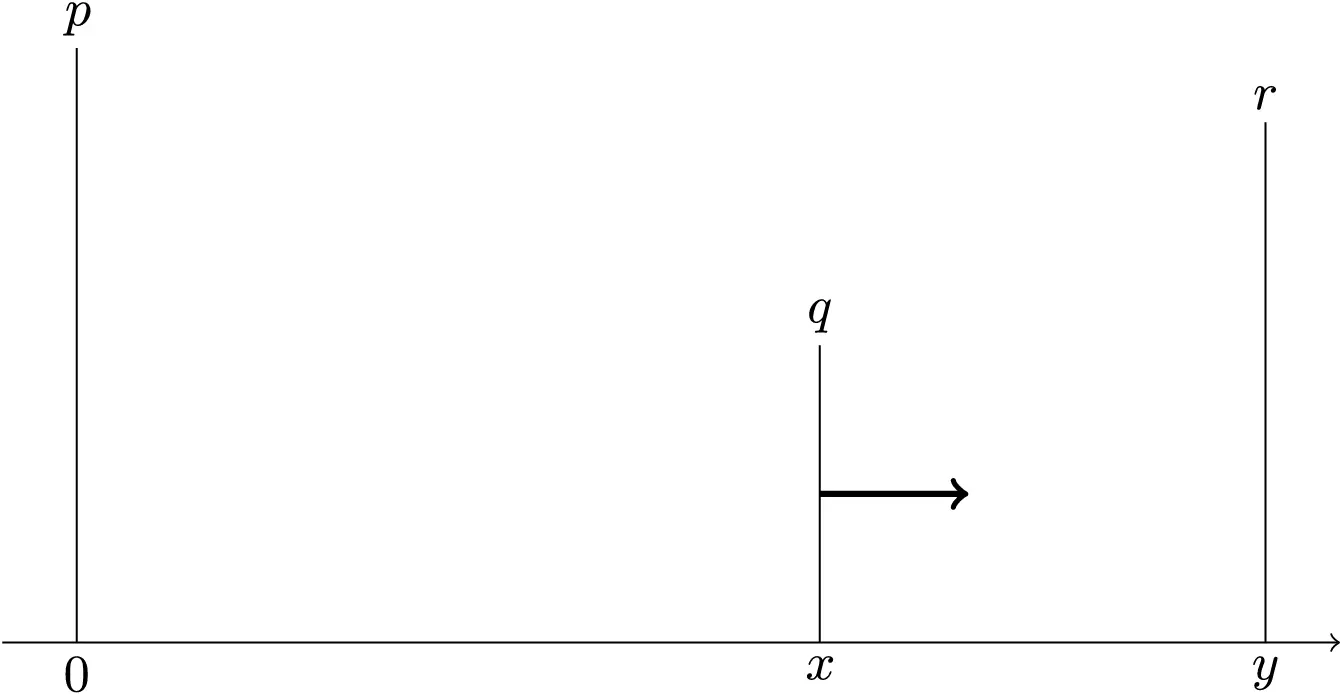
\includegraphics[height=0.16\textheight,keepaspectratio]{Images/er_axioms/axiom2.png}
    \caption{Esteban--Ray Axiom 2.}
    \label{fig:eraxiom2}
\end{figure}

\noindent This axiom captures the increased antagonism resulting from clearer separation among groups positioned at opposing extremes.

\begin{restatable}{theorem}{mecAxiomTwo}\label{th:mec-axiom-2}
The polarization measure $\MEC$ satisfies Axiom~2.
\end{restatable}

When $\beta>1$, the hypothesis $p>r$ together with $x>y-x$ forces the unique optimal consensus point $y^*$ of $\pi=((p,q,r),(0,x,y))$ to lie strictly to the left of $x$. The displacement of the middle mass from $x$ to $x+\Delta$ is therefore a shift away from consensus in the sense of Def.~\ref{def:movement}, and Th.~\ref{thm:mec-increases:body} applies.

The case $\beta=1$ requires a small additional argument. Here $x$ may itself be the unique optimal consensus point of $\pi$, in which case the shift $\pi_{x\to x+\Delta}$ is a median-shift, a situation explicitly excluded by Th.~\ref{thm:mec-increases:body}. The asymmetry $p>r$, however, is enough to ensure that even this median-shift strictly increases polarization, since by Cor.~\ref{cor:mec-special-cases} the difference reduces to $(p^\alpha-r^\alpha)\,\Delta>0$. The remaining sub-cases are non-median shifts away from consensus and so are handled by Th.~\ref{thm:mec-increases:body} as before. The full argument is given in Appendix~\ref{appendix:proof-mec-axiom-2}.


\paragraph{Axiom 3 (Dispersion to extremes).}
The third \ERLabel{} axiom says that polarization increases when central mass is redistributed symmetrically toward the two extremes.

\begin{axiom}[Polarization via dispersion to extremes]\label{axiom:3}
A polarization measure $\Pol:\Dset\to\PositiveReals$ satisfies \ERLabel{} Axiom~3 if for any $p,q>0$, any $x,y>0$ with $x=y-x$, and any $\Delta\in(0,q/2)$,
\[
\Pol((p,q,p),(0,x,y)) < \Pol((p+\Delta,q-2\Delta,p+\Delta),(0,x,y)).
\]
\begin{figure}[H]
    \centering
    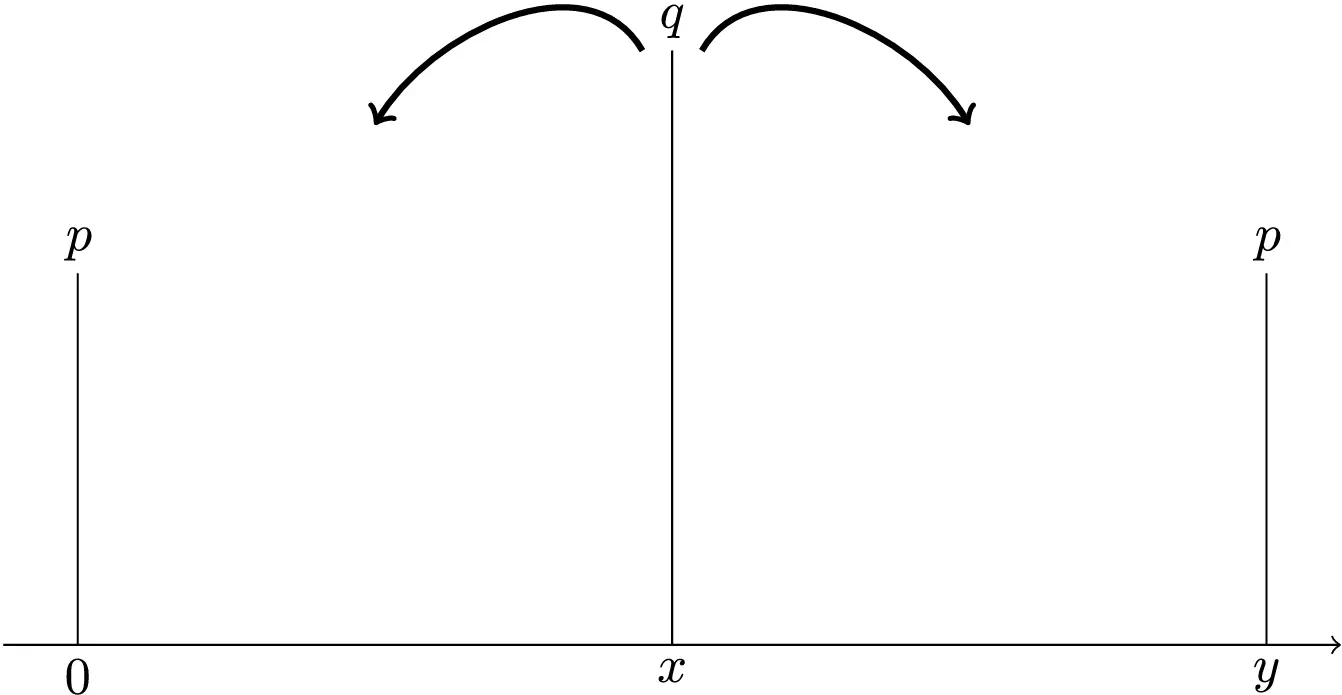
\includegraphics[height=0.16\textheight,keepaspectratio]{Images/er_axioms/axiom3.png}
    \caption{Esteban--Ray Axiom 3.}
    \label{fig:eraxiom3}
\end{figure}
\end{axiom}

\noindent This axiom reflects the intuitive notion that diminishing central positions in favor of extremes increases polarization.

\begin{restatable}{theorem}{mecAxiomThree}\label{th:mec-axiom-3}
The polarization measure $\MEC$ satisfies Axiom~3.
\end{restatable}

The argument exploits the symmetry of both distributions about $x$: by Lem.~\ref{lem:symmetry-mec}, the optimal consensus point is $x$ for both, and direct evaluation of the effort at $x$ shows the inequality.

\subsection{Central-Split Monotonicity: A New Property}\label{sec:property-1}

Beyond the three foundational axioms of Esteban and Ray, we introduce a complementary property derived as an intermediate refinement of Axiom~3.

\begin{axiom}[Central-split monotonicity, Property~1]\label{axiom:property-1}
Let \(P:\Dset\to\PositiveReals\) be a polarization measure (Def.~\ref{pol:def}). We say that \(P\) \emph{satisfies Property~1} if for any \(p,q \ge 0\), any positions \(x,y \ge 0\) and \(z>0\) satisfying \(x = y - x\) and \(x \ge z\), and any \(\Delta \in (0, q/2)\):
\[
\Pol((p,q,p), (0,x,y)) < \Pol((p, \Delta, q - 2\Delta, \Delta, p), (0,x - z, x, x + z, y)).
\]
\begin{figure}[H]
    \centering
    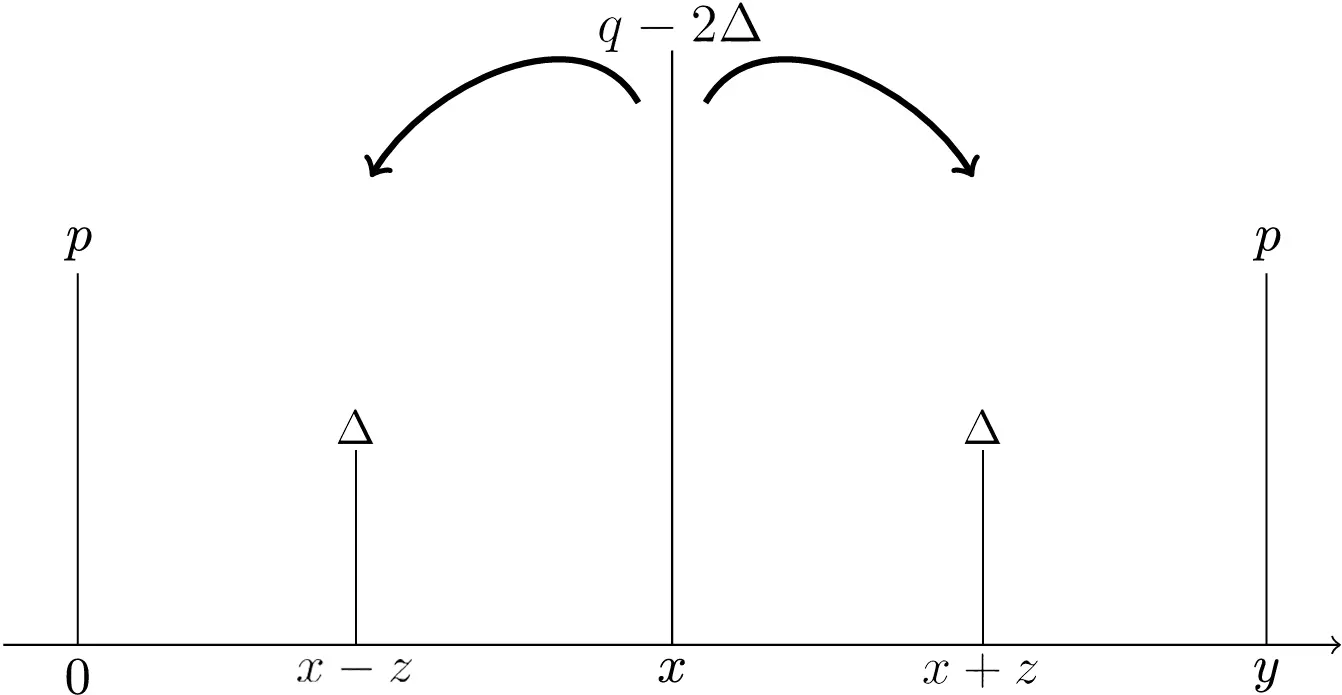
\includegraphics[height=0.16\textheight,keepaspectratio]{Images/er_axioms/property1.png}
    \caption{Property 1.}
    \label{fig:property1}
\end{figure}
\end{axiom}

\noindent Intuitively, this property indicates that polarization increases when a single central group splits into smaller groups positioned symmetrically around the original midpoint. The resulting distribution captures emerging nuances in polarization, reflecting subtle but meaningful shifts in inter-group antagonism and identification that the original Axiom~3 (which reallocates central mass directly to the extremes) does not detect.

The property is not implied by the Esteban--Ray axioms. For instance, the standard parametrization \ERLabel[0.8]{} fails it on the central-split instance obtained from
\[
((0.25,0.5,0.25),(0,0.5,1))
\]
by taking \(\Delta=0.1\) and \(z=0.1\), which gives
\[
((0.25,0.1,0.3,0.1,0.25),(0,0.4,0.5,0.6,1)).
\]
The \ERLabel[0.8]{} score decreases from approximately \(0.53\) to \(0.44\), contrary to the monotonicity required by Property~1.


\begin{restatable}{theorem}{mecPropertyOne}\label{th:mec-property-1}
For $\alpha\geq 1$ and $\beta\geq 1$, the polarization measure $\MEC$ satisfies Property~1.
\end{restatable}

The argument is similar to that of Axiom~3: by symmetry the optimal consensus point of both distributions is $x$, and direct evaluation yields the inequality.
